\section{Software Architecture Document}
\label{sec:Software Architecture Document}
Die Systemkomponenten sind in Schichten unterteilt, wobei nur eine h\"oher liegende Schicht direkten Zugriff auf eine darunterliegende Schicht hat (Schichtenarchitektur). F\"ur die Architektur lassen sich von (unten nach oben) grob die Systemkomponenten \textit{Common}, \textit{Core} und \textit{Gui} identifizieren.
% 
\begin{figure}[H]
    \centering
    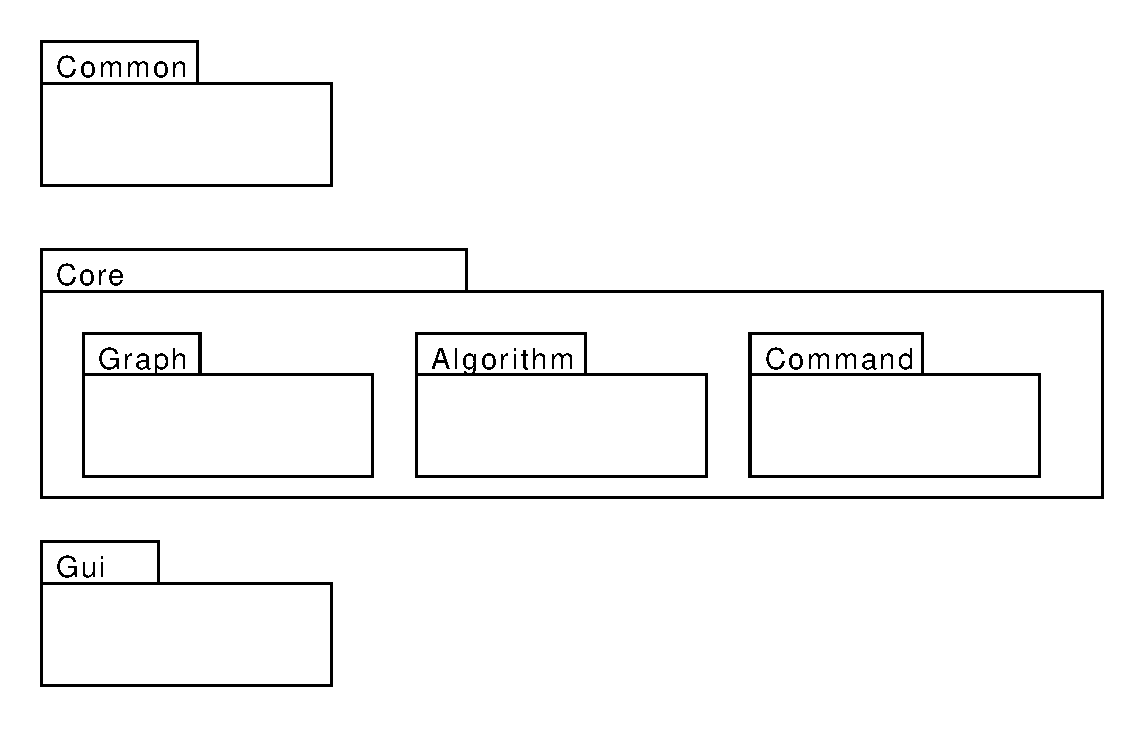
\includegraphics[scale=0.5]{diagrams/package-diagram.pdf}
    \caption{Logischen Architektur, Package Diagram}
    \label{fig:package-diagram}
\end{figure}
% 
\subsection{Common}
\label{subsec:Common}
Die Komponente h\"alt die f\"ur die Implementation eines Algorithmus zu verwendende Schnittstellen bereit. Diese sind f\"ur Algorithmen zu verwenden, welche importiert werden wollen.
% 
\subsection{Core}
\label{subsec:Core}
Die Komponente implementiert:
\begin{itemize}
  \item Data Model: Datenhaltung f\"ur Graph (Datenelemente Knoten und Kanten), Algorithmus und berechnete Traversierung (Traversierungsschritte als Operationen auf den Graphen)
  \item Business Logik: 
  \begin{itemize}
      \item Handling von Graphen und Algorithmen
      \item Traversierung und damit Erstellen der visualisierbaren L\"osung
      \item Handling von Daten-Import und L\"oschen von Daten
      \item Validierung Graphen und Algorithmen beim Import
  \end{itemize}
  \item Core Inteface: eine Schnittstelle, welche der Komponente GUI zur Verf\"ugung steht
\end{itemize}
% 
\subsection{Gui}
\label{subsec:Gui}
Die Komponente implementiert ein Model-View-Control (MVC) unter Verwendung des Java-Observer-Pattern:
\begin{itemize}
  \item Model: Observable mit s\"amtlichen GUI-Attributen und deren Getter- und Setter-Methoden
  \item View: Observer mit grafischen Elementen wie z.B. Menubar, Kn\"opfe, Regler und Text-Panelen
  \item Control: Implementiert Listeners und deren Methoden
\end{itemize}
% 
\subsubsection{Gui Elemente}
\label{subsubsec:Gui Elemente}
\begin{itemize}
  \item Daten:
  \begin{itemize}
    \item Neuen Graphen oder Algorithmus importieren
    \item Importierter Graph oder Algorithmus l\"oschen
  \end{itemize}
  \item Traversierung:
  \begin{itemize}
    \item Graph ausw\"ahlen
    \item Algorithmus ausw\"ahlen
%     \item evt. Start- resp. Endknoten ausw\"ahlen
  \end{itemize}
  \item Visualisierung:
  \begin{itemize}
      \item Einstellung Steplength: Anzahl Traversierungs-Schritte pro Bild
      \item Einstellung Delay: Zeitintervall zwischen zwei Bildern (in Sekunden)      
      \item Visualisierung, Step-by-Step: Ein Bild vor, ein Bild zur\"uck, an das Ende oder den an den Anfang springen
      \item Visualisierung, Animation: Starten, Anhalten, Stoppen
      \item Anzeige des Visualisierungsfortschrittes in einer Progressbar
  \end{itemize}
\end{itemize}
% 
\section{Development Environment}
\label{sec:Development Environment}
Das System wird in der Programmiersprache Java implementiert. Es werden das Java Universal Network/Graph Framework (JUNG, \url{http://jung.sourceforge.net/}), das XML-basierte Format GraphML (\url{http://graphml.graphdrawing.org/}), die Apache Commons IO Library und das Java Swing Framework verwendet. F\"ur das Sourcecode Management (SCM) wird die Software git verwendet. Als IDE kommt Eclipse mit EGit zum Einsatz.

Das Projekt wird auf github verwaltet. Urspr\"unglich war es erreichbar unter \url{https://github.com/brugr9/ch.bfh.bti7301.hs2013.GraphVisualisierung2} (wird bis nach Erhalt der Bewertung des Projektes nicht gel\"oscht). Seit dem Entscheid in der Woche 45, das Projekt mit Maven zu erweitern, wird das Projekt jedoch unter \url{https://github.com/brugr9/gravis} weitergef\"uhrt.